% !TEX root = ../main.tex

% ---------------------------------------------------------------
% Automatic generation of a self-adaptive TLM model
% ---------------------------------------------------------------

\chapter[Apprendimento non supervisionato]{Apprendimento non supervisionato per l'identificazione di contensti di FoG}\label{chap5:Automatic}
I lavori che sono stati svolti e presentati nel capitolo \ref{chap2:related} sul Freezing Of Gait sono basati su approcci di classificazione ossia, come spiegato nel capitolo \ref{chap3:background}, allenano un algoritmo con dei dataset di training nel quale le etichette di ogni istante vengono fornite dalla supervisione di un dottore o fisioterapista e poi, tale algoritmo allenato, viene testato su dei nuovi dati al fine di rilevare i contesti di FoG. Il lavoro che viene presentato in questo capitolo, invece, usa le etichette fornite dal dataset solo come confronto ai risultati forniti dagli algoritmi di clustering. Quest'ultimi, infatti, una volta forniti i dati o feature (proprietà) su cui voglia applicarli, restituiscono, per ogni osservazione(nel nostro caso riga del dataset), un'etichetta che indica a quale contesto è stato assegnato ogni dato, se di FoG, non-FoG o Pre-FoG.\\
Innanzitutto verrà fornita una descrizione del dataset utilizzato e di come è stato modificato per le nostre esigenze. Verranno poi descritti i metodi utilizzati dall'approccio scelto e viene fornito il codice implementativo. Tutte lo sviluppo è stato effettuato tramite software Matlab \footnote{https://it.mathworks.com/products/matlab.html}.
\section{Dataset}
L'approccio che andiamo a proporre è stato testato sul dataset DAPHNET\footnote{www.wearable.ethz.ch/resources/Dataset}, il quale contiene dati collezionati da 10 pazienti parkinsoniani, dei quali 8 presentano contesti di FoG, mentre 2 di loro non ne presentano. I dati sono stati registrati usando 3 accelerometri 3D attaccati alla caviglia, al ginocchio e nella zona lombare del paziente, usando una frequenza di campionamento di 64 Hz, ossia vengono raccolti 64 campioni ogni secondo.\\
I soggetti hanno completato sessioni da 20-30 minuti ciascuno, consistenti di 3 fasi di camminata:
\begin{enumerate}
	\item Camminata avanti ed indietro lungo una linea retta, con delle rotazioni di 180 gradi;
	\item Camminata casuale con una serie di fermate volontarie e rotazioni di 360 gradi;
	\item Camminata che simula attività di vita quotidiana, tra le quali entrare in stanze ed uscirne, camminare nella cucina, prendersi un bicchiere d'acqua e tornare al punto di partenza.
\end{enumerate}
Le prestazioni motorie variano molto tra i pazienti. Mentre alcuni soggetti hanno mantenuto una camminata regolare durante gli episodi di non FoG, altri hanno camminato molto lentamente ed in modo instabile. L'intero dataset contiene in totale 237 episodi di FoG; la durata di ognuno di essi è tra i 0.5s ed i 40.5s. Il 50\% degli episodi di FoG è durato meno di 5.4s ed il 93.2\% è più corto di 20s. Gli episodi di FoG sono stati identificati da fisioterapisti usando registrazioni video sincronizzate. L'inizio di un episodio di FoG è stato definito come il punto dove la sequenza normale di camminata è stata interrotta, mentre la fine del FoG è stata definita come il momento in cui tale sequenza riprende.\\
Per il lavoro svolto nella tesi, oltre alle etichette date dai dottori nei casi di non FoG e FoG, abbiamo introdotto nei dati una nuova label, che indica il momento che noi indichiamo come pre-FoG, per cui tutti i campioni precedenti ad un'occorrenza di FoG sono stati etichettati con questa nuova label. Quindi ci ritroviamo con 3 label diverse invece di 2 (tutti i lavori in letteratura rientrano nell'ultimo caso): l'etichetta 1 indica un No-FoG, la label 2 indica un FoG, l'etichetta 3 indica invece un pre-FoG.
\section{Approccio basato su Feature Statistiche}
I dati raccolti dagli accelerometri, se presi in forma grezza, hanno poca potenza espressiva, ossia non riescono a fornire molte informazioni su ciò che stiamo cercando (contesti di FoG), quindi si rende necessaria una rimodellazione di tali dati. Il primo approccio che è stato preso in considerazione è basato sul calcolo di feature ( o proprietà) basate su grandezze che provengono dalla matematica statistica. Il flusso di tale approccio è:
\begin{enumerate}
	\item Pre-processamento dei dati degli accelerometri, al fine di eliminare il rumore presente ed identificare eventuali punti di outline, ossia campioni che non presentano affinità col resto dei dati poiché dovuti a movimenti non consoni;
	\item Finestramento dei dati in base ad intervalli variabili al fine di calcolare le feature, dove ogni intervallo presenta una certa sovrapposizione con l'intervallo precedente;
	\item Calcolo effettivo delle feature statistiche;
	\item Applicazione degli algoritmi di clustering;
	\item Calcolo di metriche che indicano quanto bene gli algoritmi di clustering hanno lavorato in relazione alle label fornite dal dataset.
\end{enumerate}
\subsection{Pre-processamento dei dati}
Gli accelerometri sono dispositivi che misurano le vibrazioni o l'accelerazione del movimento di una struttura. La forza generata dalle vibrazioni o una variazione del movimento (accelerazione) fa in modo che la massa "comprima" il materiale piezoelettrico, che genera una carica elettrica proporzionale alla forza esercitata su di esso. Dato che la carica è proporzionale alla forza e che la massa è una costante, la carica è proporzionale anche all'accelerazione. Come tutti i dispositivi che misurano delle grandezze presentano dell'incertezza strumentale che può portare ad avere rumore, ossia un segnale non desiderato, di origine naturale o artificiale, che si sovrappone all'informazione degli accelerometri stessi. QUesto rumore porta ad avere dei punti definiti outlier, ossia campioni che non presentano affinità col resto dei dati poiché dovuti a movimenti non consoni.\\
Al fine di rimuovere tali punti, che altererebbero in modo negativo il calcolo delle nostre feature, si rende necessario rimuoverli dal nostro dataset. Per identificarli, è stato implementato un filtro passa-alto che eliminano tutte le frequenze inferiori a 0.5Hz, le quali non appartengono al normale movimento umano ma indicano appunto la presenza di rumore, come evidenziato in \cite{21}. L'implementazione del filtro viene fornita in \ref{hpfilter}.
\begin{lstlisting}[frame=single, caption=hpfilter, label=hpfilter]  % Start your code-block
function Hd = hpfilter
% All frequency values are in Hz.
Fs = 64;  % Sampling Frequency

Fstop = 0.4;    % Stopband Frequency
Fpass = 0.8;       % Passband Frequency
Astop = 60;      % Stopband Attenuation (dB)
Apass = 1;       % Passband Ripple (dB)
match = 'passband';  % Band to match exactly

% Construct an FDESIGN object and call its ELLIP method.
h  = fdesign.highpass(Fstop, Fpass, Astop, Apass, Fs);
Hd = design(h, 'cheby2', 'MatchExactly', match);
\end{lstlisting}
\subsection{Definizione degli intervalli}

\subsection{Calcolo delle Feature}
 Le feature prese in considerazione nel nostro studio sono descritte in tabella \ref{TAB:Feature}.
\begin{table}[h!]
	\begin{tabular}{ |p{0.05\textwidth} | p{0.25\textwidth} | p{0.6\textwidth} | }
		\multicolumn{1}{|p{0.05\textwidth} |}{\textbf{N}} &  
		\multicolumn{1}{p{0.25\textwidth} |}{\textbf{Feature}} &
		\multicolumn{1}{p{0.6\textwidth} |}{\textbf{Descrizione}}\\
		\hline
		\hline
		1 & Minimo & Valore minimo del segnale\\
		2 & Massimo & Valore massimo del segnale \\
		3 & Mediana & Valore mediano del segnale \\
		4 & Media & Valore medio del segnale \\
		5 & Media Armonica & Media armonica del segnale \\
		6 & Errore Quadratico Medio & Valore Quadratico medio del segnale \\
		7 & Media Geometrica & Media geometrica del segnale \\
		8 & Varianza & Radice della deviazione standard \\
		9 & Deviazione Standard & Deviazione media del segnale rispetto alla media \\
		10 & Curtosi & Allontanamento dalla normalità distributiva del segnale \\
		11 & Simmetria & Grado di asimmetria della distribuzione del segnale \\
		12 & Moda & Il numero che appare più volte nel segnale \\
		13 & Media Tagliata & Media tagliatadel segnale nella finestra \\
		14 & Entropia & Misura della di distruzione delle componenti in frequenza \\
		15 & Range & Differenza tra il valore minimo e massimo del segnale \\
		16 & Magnitudine & Somma della norma euclidea di tre assi normalizzato sulla lunghezza del segnale \\
		17 & Area Magnitudine & Accelerazione della magnitudine di tre assi normalizzato sulla lunghezza del segnale \\
		18 & Autovalori delle direzioni dominanti & Autovalori della matrice di covarianza di tre assi \\
		19 & Accelerazione media dell'energia & Valore medio dell'energia sui 3 assi \\
	\end{tabular}
\caption{Descrizione delle Feature Statistiche}
\label{TAB:Feature}
\end{table}\\
Prima di calcolare tali feature, però, è necessario pre-processare i dati in modo da eliminare il più possibile il rumore presente o gli outlier,  A tale scopo, è stato progettato un filtro passa banda in modo da eliminare tutti i movimenti che presentano una frequenza inferiore a 0.5Hz o superiore a 20Hz, in accordo con \cite{21}, dato che il movimento umano è compreso tra questi due valori.\\
Una volta filtrati i dati, il passo successivo è scegliere l'intervallo della finestra temporale su cui calcolare le feature. Questa però non ha una lunghezza definita a priori in letteratura, per cui abbiamo condotto uno studio su quale fosse la migliore scelta. Inoltre, poiché non vogliamo perdere determinati movimenti tra una finestra e l'altro, per cui si è deciso di fare sovrapposizione tra finsetre. Anche questo parametro non è definito a priori, per cui anche questo valore è stato fatto variare e condotto un studio su quale fosse il migliore. I range su cui sono stati fatti i test sono: da 1 a 5 secondi per quanto riguarda la dimensione della finestra temporale, da 0.5 a 4.5 secondi invece per l'intervallo di soprapposizione, con la condizione che il tempo di sovrapposizione sia sempre minore di quello della finestra. Per esempio, poiché ho una frequenza di campionamento di 64 Hz, scegliendo 2 secondi come intervallo della finestra e 0.5 secondi di overlap, avrò che la prima finestra va dal campione 1 al campione 129, la seconda finestra va dal campione 98 al campione 226, la terza finestra dal campione 195 al campione 323 e così via. L'intervallo che invece è stato definito a priori è quello relativo al pre-fog, che è stato posto a 2s in accordo con \cite{12}.
\begin{figure}[h!]
	\centering
	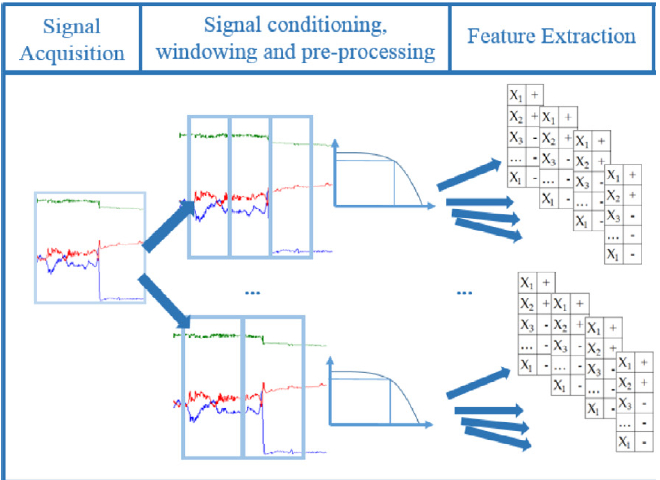
\includegraphics[scale=0.6]{images/flusso_feature.png}
	\caption{Schema generale di calcolo delle feature statistiche}
	\label{Flusso Feature}
\end{figure}
Per ogni combinazione di finestra temporale, quindi, vengono calcolate le rispettive feature e si procede ad applicare l'algoritmo di clustering. Quelli che sono stati scelti, in quanto più diffusi nel contesto di clustering, sono: k-means, self-organizing map e fuzzy c-means. Il k-means viene testato con tutte le sue metriche di distanza, per evidenziare eventuali differenze e decidere quale tra le 4 presenti (cosine, euclidean, cityblock, correlation) si adatta di più al nostro problema. Il fuzzy c-means è stato scelto anche perché è di soft clustering, ossia 2 punti potrebbero appartenere a 2 cluster diversi, il che ritorna utile nel trovare correttamente la terza label, in quanto nel dataset originale era etichettata con una diversa label.\\
Ogni algoritmo di clustering restituisce un vettore di etichette, che indicano il numero di cluster a cui è stato assegnato ogni punto. Questi vengono messi a confronto con le true label, ossia le etichette inserite a mano dal dottore, e si calcolano le metriche di accuratezza, precisione, sensitività e F1-measure attraverso la matrice di confusione descritta precedentemente. Le true label vengono calcolate, per ogni vettore di feature, come la moda tra le label della finestra temporale, ossia come l'etichetta che si presente più volte all'interno della finestra stessa. Una volta ottenute le misure per tutti i campioni temporali, si cercano gli intervalli con il maggiore punteggio, dove con quest'ultimo intendiamo la media delle 4 grandezze calcolate. Nel nostro caso, come si vede nella figura \ref{SecondiOverlap}, abbiamo che i punteggi migliori vengono raggiunti nell'intervallo compreso tra 1.5 e 2 secondi, con una sovrapposizione di 0.5 o 1 secondo. Dato che nella maggior parte dei casi risultano tali intervalli, decidiamo di concentrarci su questi, anche perché sono accettabili in un'implementazione online. Nella figura \ref{Accuratezza} si può vedere il valore di accuratezza per ogni paziente per i vari algoritmi di clustering, mentre nella figura \ref{Precisione} possiamo osservare la precisione per ogni paziente ed infine nella figura \ref{Recall} si può vedere il valore di recall per ogni algortimo e paziente.
\begin{figure}[]
	\centering
	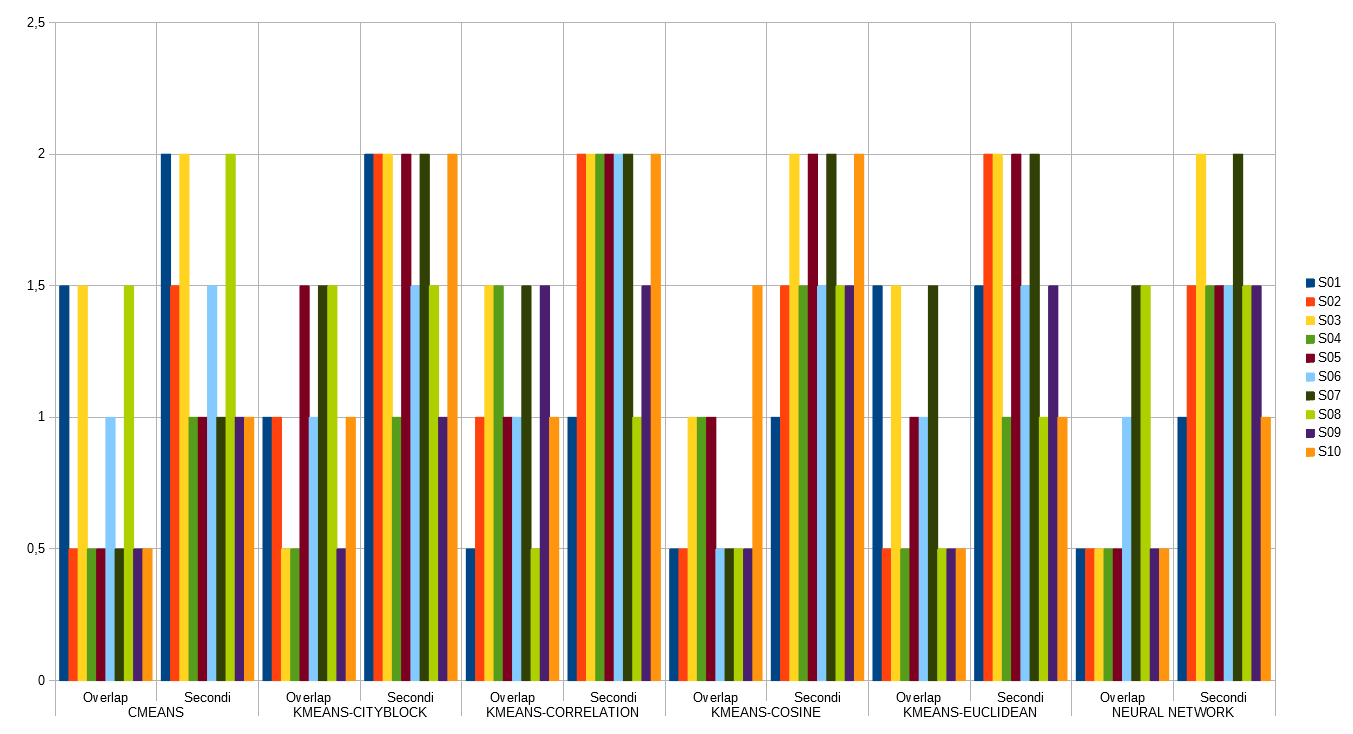
\includegraphics[scale=0.35]{images/secondi_overlap.png}
	\caption{Grafico degli intervalli di overlap e secondi della finestra temporale per ogni paziente}
	\label{SecondiOverlap}
\end{figure}

\begin{figure}[]
	\centering
	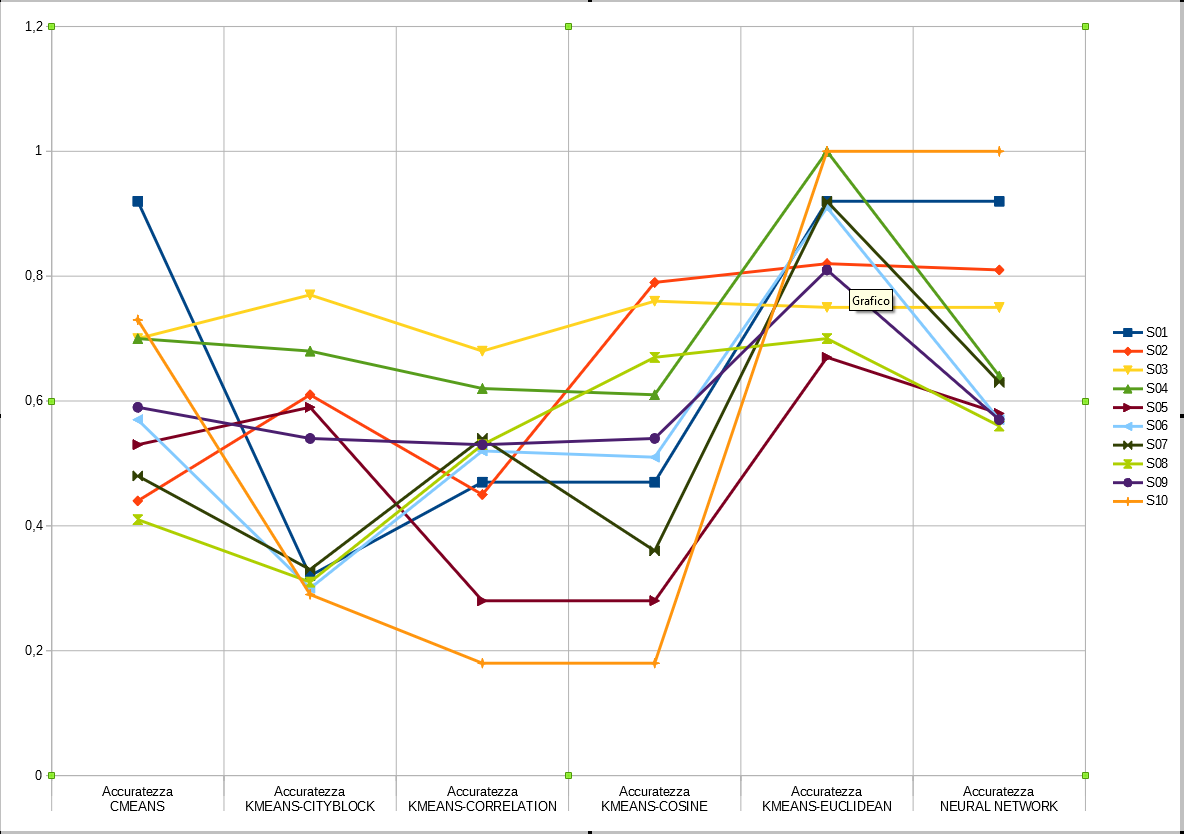
\includegraphics[scale=0.35]{images/accuratezza.png}
	\caption{Grafico dell'accuratezza per ogni paziente}
	\label{Accuratezza}
\end{figure}
\begin{figure}[]
	\centering
	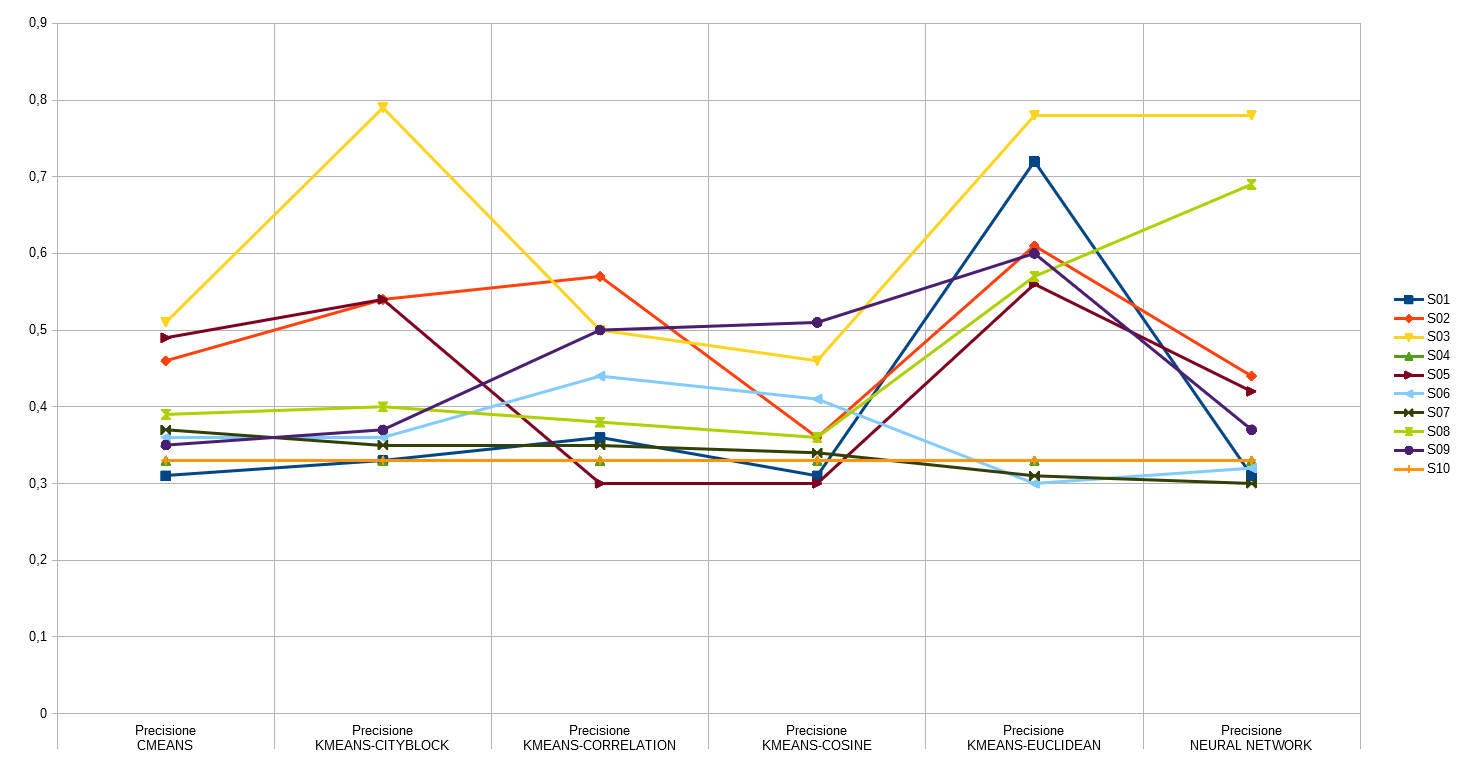
\includegraphics[scale=0.3]{images/precisione.png}
	\caption{Grafico della precisione media delle classi per ogni paziente}
	\label{Precisione}
\end{figure}
\begin{figure}[]
	\centering
	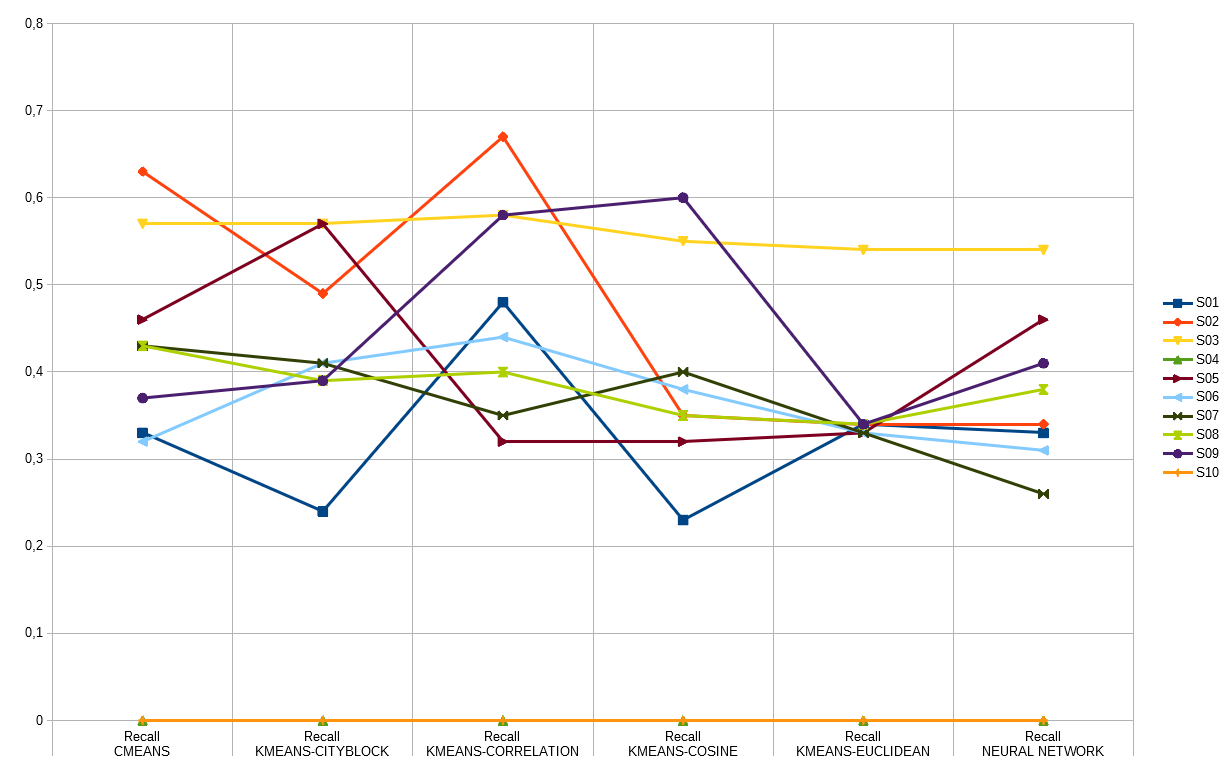
\includegraphics[scale=0.35]{images/recall.png}
	\caption{Grafico della recall media delle classi per ogni paziente}
	\label{Recall}
\end{figure}
Oltre a determinare le migliori combinazioni secondi-overlap, siamo stati in grado di verificare quale metrica dell'algoritmo di clustering k-means meglio si adatta ai nostri dati. Infatti, nella figura \ref{Accuratezza} possiamo vedere che la metrica Euclidean ha in media il valore più alto rispetto alle altre, anche se questo, osservando le figure \ref{Precisione} e \ref{Recall}, è dato dal fatto che sbaglia meno volte rispetto alle altre metriche ad etichettare il NoFog e, essendo questa label in quantità maggiore rispetto alle altre, porta ad un'accuracy totale più alta.\\

\section{Feature Dinamiche}


\section{Linear Discriminant Analysis}












%\begin{table}[htp]
%	\centering
%	\begin{tabular}{lllll}
%		Tutti & CMEANS &  &  &  \\
%		Paziente & Accuratezza & Precisione & Recall & F1-measure \\
%		S01 & 0,92 & 0,31 & 0,33 & 0,32 \\
%		& 1 & 2,50 & 0,00 & 0,00 \\
%		S02 & 0,44 & 0,46 & 0,63 & 0,53 \\
%		& 0,50 & 2,00 & 0,00 & 0,00 \\
%		S03 & 0,70 & 0,51 & 0,57 & 0,54 \\
%		& 1 & 2 & 0,00 & 0,00 \\
%		S04 & 0,70 & 0,33 & 0,00 & 0,00 \\
%		& 0,50 & 2 & 0,00 & 0,00 \\
%		S05 & 0,53 & 0,49 & 0,46 & 0,47 \\
%		& 0,50 & 1,50 & 0,00 & 0,00 \\
%		S06 & 0,57 & 0,36 & 0,32 & 0,34 \\
%		& 1,00 & 1,50 & 0,00 & 0,00 \\
%		S07 & 0,48 & 0,37 & 0,43 & 0,40 \\
%		& 0,50 & 2,00 & 0,00 & 0,00 \\
%		S08 & 0,41 & 0,39 & 0,43 & 0,41 \\
%		& 1,50 & 2,50 & 0,00 & 0,00 \\
%		S09 & 0,59 & 0,35 & 0,37 & 0,36 \\
%		& 1,50 & 2,00 & 0,00 & 0,00 \\
%		S10 & 0,73 & 0,33 & 0,00 & 0,00 \\
%		& 1 & 2 & 0,00 & 0,00
%	\end{tabular}
%	\caption{Rate Pazienti per l'algoritmo di clustering C-means}
%	\label{ratecmeans}
%\end{table}
%\begin{table}[htp]
%	\centering
%	\begin{tabular}{lllll}
%		Tutti & \multicolumn{4}{c}{KMEANS-CITYBLOCK} \\
%		Paziente & Accuratezza & Precisione & Recall & F1-measure \\
%		S01 & 0,32 & 0,33 & 0,24 & 0,28 \\
%		& 1,00 & 2,50 & 0,00 & 0,00 \\
%		S02 & 0,61 & 0,54 & 0,49 & 0,51 \\
%		& 1,00 & 2,00 & 0,00 & 0,00 \\
%		S03 & 0,77 & 0,79 & 0,57 & 0,66 \\
%		& 0,50 & 2,00 & 0,00 & 0,00 \\
%		S04 & 0,68 & 0,33 & 0,00 & 0,00 \\
%		& 0,50 & 1,00 & 0,00 & 0,00 \\
%		S05 & 0,59 & 0,54 & 0,57 & 0,55 \\
%		& 1,00 & 2,00 & 0,00 & 0,00 \\
%		S06 & 0,30 & 0,36 & 0,41 & 0,38 \\
%		& 1,00 & 2,00 & 0,00 & 0,00 \\
%		S07 & 0,33 & 0,35 & 0,41 & 0,38 \\
%		& 1,50 & 2,50 & 0,00 & 0,00 \\
%		S08 & 0,31 & 0,40 & 0,39 & 0,40 \\
%		& 1,50 & 2,00 & 0,00 & 0,00 \\
%		S09 & 0,54 & 0,37 & 0,39 & 0,38 \\
%		& 0,50 & 2,00 & 0,00 & 0,00 \\
%		S10 & 0,29 & 0,33 & 0,00 & 0,00 \\
%		& 1,00 & 2,00 & 0,00 & 0,00
%	\end{tabular}
%	\caption{Rate Pazienti per l'algoritmo di clustering K-means con metrica di distanza Cityblock}
%	\label{ratekmeanscityblock}
%\end{table}
%\begin{table}[]
%	\centering
%	\begin{tabular}{lllll}
%		Tutti & \multicolumn{4}{c}{KMEANS-CORRELATION}  \\
%		Paziente & Accuratezza & Precisione & Recall & F1-measure \\
%		S01 & 0,47 & 0,36 & 0,48 & 0,41 \\
%		& 0,50 & 2,00 & 0,00 & 0,00 \\
%		S02 & 0,45 & 0,57 & 0,67 & 0,62 \\
%		& 1,00 & 2,50 & 0,00 & 0,00 \\
%		S03 & 0,68 & 0,50 & 0,58 & 0,54 \\
%		& 1,00 & 2,50 & 0,00 & 0,00 \\
%		S04 & 0,62 & 0,33 & 0,00 & 0,00 \\
%		& 1,50 & 2,00 & 0,00 & 0,00 \\
%		S05 & 0,28 & 0,30 & 0,32 & 0,31 \\
%		& 1,00 & 2,00 & 0,00 & 0,00 \\
%		S06 & 0,52 & 0,44 & 0,44 & 0,44 \\
%		& 1,00 & 2,00 & 0,00 & 0,00 \\
%		S07 & 0,54 & 0,35 & 0,35 & 0,35 \\
%		& 1,50 & 2,50 & 0,00 & 0,00 \\
%		S08 & 0,53 & 0,38 & 0,40 & 0,39 \\
%		& 0,50 & 2,00 & 0,00 & 0,00 \\
%		S09 & 0,53 & 0,50 & 0,58 & 0,54 \\
%		& 1,50 & 2,00 & 0,00 & 0,00 \\
%		S10 & 0,18 & 0,33 & 0,00 & 0,00 \\
%		& 1,00 & 2,50 & 0,00 & 0,00
%	\end{tabular}
%	\caption{Rate Pazienti per l'algoritmo di clustering K-means con metrica di distanza Correlation}
%	\label{ratekmeanscorrelation}
%\end{table}
%\begin{table}[]
%	\centering
%	\begin{tabular}{lllll}
%		Tutti & \multicolumn{4}{c}{KMEANS-COSINE} \\
%		Paziente & Accuratezza & Precisione & Recall & F1-measure \\
%		S01 & 0,47 & 0,31 & 0,23 & 0,27 \\
%		& 0,50 & 2,00 & 0,00 & 0,00 \\
%		S02 & 0,79 & 0,36 & 0,35 & 0,35 \\
%		& 0,50 & 1,50 & 0,00 & 0,00 \\
%		S03 & 0,76 & 0,46 & 0,55 & 0,50 \\
%		& 1,00 & 2,00 & 0,00 & 0,00 \\
%		S04 & 0,61 & 0,33 & 0,00 & 0,00 \\
%		& 1,00 & 1,50 & 0,00 & 0,00 \\
%		S05 & 0,28 & 0,30 & 0,32 & 0,31 \\
%		& 1,00 & 2,50 & 0,00 & 0,00 \\
%		S06 & 0,51 & 0,41 & 0,38 & 0,40 \\
%		& 0,50 & 1,50 & 0,00 & 0,00 \\
%		S07 & 0,36 & 0,34 & 0,40 & 0,37 \\
%		& 0,50 & 2,00 & 0,00 & 0,00 \\
%		S08 & 0,67 & 0,36 & 0,35 & 0,35 \\
%		& 1,00 & 1,50 & 0,00 & 0,00 \\
%		S09 & 0,54 & 0,51 & 0,60 & 0,55 \\
%		& 1,00 & 2,00 & 0,00 & 0,00 \\
%		S10 & 0,18 & 0,33 & 0,00 & 0,00 \\
%		& 2,00 & 2,50 & 0,00 & 0,00
%	\end{tabular}
%	\caption{Rate Pazienti per l'algoritmo di clustering K-means con metrica di distanza Cosine}
%	\label{ratekmeanscosine}
%\end{table}
%\begin{table}[]
%	\centering
%	\begin{tabular}{lllll}
%		Tutti & \multicolumn{4}{c}{KMEANS-EUCLIDEAN} \\
%		Paziente & Accuratezza & Precisione & Recall & F1-measure \\
%		S01 & 0,92 & 0,72 & 0,34 & 0,46 \\
%		& 1,50 & 2,00 & 0,00 & 0,00 \\
%		S02 & 0,82 & 0,61 & 0,34 & 0,44 \\
%		& 0,50 & 2,50 & 0,00 & 0,00 \\
%		S03 & 0,75 & 0,78 & 0,54 & 0,64 \\
%		& 1,50 & 2,50 & 0,00 & 0,00 \\
%		S04 & 1,00 & 0,33 & 0,00 & 0,00 \\
%		& 0,50 & 2,00 & 0,00 & 0,00 \\
%		S05 & 0,67 & 0,56 & 0,33 & 0,42 \\
%		& 1,00 & 2,00 & 0,00 & 0,00 \\
%		S06 & 0,91 & 0,30 & 0,33 & 0,32 \\
%		& 1,00 & 1,50 & 0,00 & 0,00 \\
%		S07 & 0,92 & 0,31 & 0,33 & 0,32 \\
%		& 2,00 & 2,50 & 0,00 & 0,00 \\
%		S08 & 0,70 & 0,57 & 0,34 & 0,42 \\
%		& 0,50 & 1,00 & 0,00 & 0,00 \\
%		S09 & 0,81 & 0,60 & 0,34 & 0,43 \\
%		& 0,50 & 2,00 & 0,00 & 0,00 \\
%		S10 & 1,00 & 0,33 & 0,00 & 0,00 \\
%		& 0,50 & 2,00 & 0,00 & 0,00
%	\end{tabular}
%	\caption{Rate Pazienti per l'algoritmo di clustering K-means con metrica di distanza Euclidean}
%	\label{ratekmeanseuclidean}
%\end{table}
%\begin{table}[]
%	\centering
%	\begin{tabular}{lllll}
%		Tutti & \multicolumn{4}{c}{NEURAL NETWORK} \\
%		Paziente & Accuratezza & Precisione & Recall & F1-measure \\
%		S01 & 0,92 & 0,31 & 0,33 & 0,32 \\
%		& 0,50 & 2,00 & 0,00 & 0,00 \\
%		S02 & 0,81 & 0,44 & 0,34 & 0,38 \\
%		& 0,50 & 1,50 & 0,00 & 0,00 \\
%		S03 & 0,75 & 0,78 & 0,54 & 0,63 \\
%		& 0,50 & 2,50 & 0,00 & 0,00 \\
%		S04 & 0,64 & 0,33 & 0,00 & 0,00 \\
%		& 0,50 & 2,00 & 0,00 & 0,00 \\
%		S05 & 0,58 & 0,42 & 0,46 & 0,44 \\
%		& 0,50 & 2,00 & 0,00 & 0,00 \\
%		S06 & 0,57 & 0,32 & 0,31 & 0,31 \\
%		& 1,00 & 1,50 & 0,00 & 0,00 \\
%		S07 & 0,63 & 0,30 & 0,26 & 0,28 \\
%		& 2,00 & 2,50 & 0,00 & 0,00 \\
%		S08 & 0,56 & 0,69 & 0,38 & 0,49 \\
%		& 1,50 & 2,00 & 0,00 & 0,00 \\
%		S09 & 0,57 & 0,37 & 0,41 & 0,39 \\
%		& 0,50 & 2,00 & 0,00 & 0,00 \\
%		S10 & 1,00 & 0,33 & 0,00 & 0,00 \\
%		& 0,50 & 1,00 & 0,00 & 0,00
%	\end{tabular}
%	\caption{Rate Pazienti per l'algoritmo di clustering Self-Organizing Map}
%	\label{rateneuralnetwork}
%\end{table}